% !TeX spellcheck = en_GB
%Introduction
%\begin{savequote}[50mm]
%If our brains were simple enough for us to understand them, we'd be so simple that we couldn't.
%\qauthor{Ian Stewart }%The Collapse of Chaos: Discovering Simplicity in a Complex World
%\end{savequote}
\chapter{Background and Related Work}
\label{chap:sota}

\section{Overview}
As explained in Section \ref{motivation}, there is a new trend towards hybrid broadcast-broadband multi-device services which are not still easy to develop for broadcasters and application developers due to a lack of rules or hints to select the best user interface based on some contextual factors. To provide the basis of the research that overcomes that challenge, this chapter is divided in three sections. Section \ref{hybridEc} and Section \ref{mdTech} gather the background of the hybrid TV ecosystem and the technologies for interoperable multi-device services respectively, while Section \ref{UIOpt} describes the related work regarding the optimisation of the user interface in multi-device media services. This last section goes over previous work dedicated to multi-device or multi-content optimisation in similar environments like the target one to be able to identify the unsolved problems. 
\section{Analysis of the hybrid TV ecosystem}\label{hybridEc}

This subsection presents an analysis of the environment and technologies involved focusing on Hybrid broadcast-Internet multi-device services. The following is a list of statistics and facts about the hybrid ecosystem.
\begin{enumerate}
	\item Future of Broadcast Television Initiative (FOBTV) was founded in 2012 by broadcasters, manufacturers, network operators, standardisation organisations, research institutes and universities around the world, aimed primarily at developing requirements for next-generation TV where new services with smart interaction and personalisation are becoming more and more relevant \cite{Zang2014}.
	\item Broadcast capable devices are still the most used for the consumption of media services and thus, the most appropriate to reach a higher audience. According to the Nielsen report of Q3 2018 \cite{nielsen2018}, TV and radio account for 57\% of the average audience among adults aged 18+.
	\item Smart TV shipments \cite{statistaWeb} have constantly increased over the years. From the 109.3 Million Smart TVs shipped in 2014, this increased to 240.2 Million in 2018 and reached 265.3 Million in 2019.
	%\item HbbTV market penetration \cite{jurgen2016} is continuously rising and the majority of western European countries have vigorously adopted this standard where more than the 70\% of TVs sold are HbbTV. There are 43 Million available devices with HbbTV 1.5 being the most widespread version, as HbbTV 2.0 is not included in many of the commercial devices as yet. Furthermore, in the USA the Advanced Television Systems Committee (ATSC), is working on the ATSC 3.0 standard \cite{ATSC3} and will be liaising actively with HbbTV to use HbbTV 2.0 as part of it \cite{flier}.Moreover, Operator Applications (OpApps) \cite{opapp} specification is an extension to the core HbbTV specification to support operator application. It describes how the HbbTV browser can run both HbbTV broadcaster applications and operator applications at the same time.
	\item According to the TV and Media study \cite{ericsson16} by Ericsson ConsumerLab , in 2016, 31\% of users browsed Internet content related to what they were watching, 19\% of users participated in online discussions about the content being watched, and lastly, 20\% of users used the second screen to watch two or more programs at the same time. Those percentages were 23\%, 17\% and 15\% respectively in 2014. Moreover, according to the same study in 2017 \cite{ericsson17} in 2020, it is expected that only 1 in 10 consumers to be stuck watching TV only on a traditional screen, a 50 percent decrease compared to 2010. Therefore consumers are evolving into higher-usage and higher-spending multi-screen viewers. 
\end{enumerate}

From the above facts we can conclude that although there is not too much experience around hybrid multi-device experiences, the market shows a clear trend towards them. 

For that, there are broadcast-broadband standards and specifications that provide interactive experiences within Digital TV, providing solutions to add second screen devices to the experience in cooperation with the TV.

Nested Context Language (NCL) \cite{soares2009multiple} is the declarative language of the Brazilian Terrestrial Digital TV System supported by its middleware called Ginga. NCL is standardised in the ITU-T Recommendation H.761 for IPTV services. As a glue language, NCL relates media objects in time and space without restricting or imposing any media content type, including media objects with imperative and declarative code written using other languages \cite{soares2010ginga}. Moreover, NCL provides declarative support for presenting distributed DTV applications on multiple devices. Presentation of media objects in NCL applications can be associated to devices using an abstraction called device classes and the parent device, for instance the TV, controls the secondary devices. \cite{soares2009multiple} presents a solution for the exhibition of multiple devices in cooperation in DTV Systems with NCL.

HbbTV is a pan-European specification published by ETSI to allow broadcasters signalling, delivery through the carousel, rendering and controlling the application with a HTML based browser in the TV or set-top box, providing a hybrid broadcast-broadband experience \cite{merkel2011hybrid}. In February 2015, the 2.0 \cite{hbbtv20} specification of HbbTV  was published with new functionalities. In contrast with versions 1.0 \cite{hbbtv10}/1.5 \cite{hbbtv15}, HbbTV 2.0 uses HTML5 and a set of related Web technologies including many modules from CSS level 3, DOM level 3, Web Sockets, etc. Regarding the addition of companion screens to the TV, an HbbTV 2.0 application on a TV can launch an application on a suitably enabled mobile device. Moreover, HbbTV 2.0 enables an application on mobile to remotely launch an HbbTV application on a TV, based on DIAL \cite{dial}.

HbbTV has come about as a combination of different standards in order to develop and promote open specifications and solutions for hybrid broadcast-broadband and IPTV television systems, with the aim of allowing harmonisation of broadcast and broadband delivered entertainment services and consumer equipment. 


\begin{figure}
	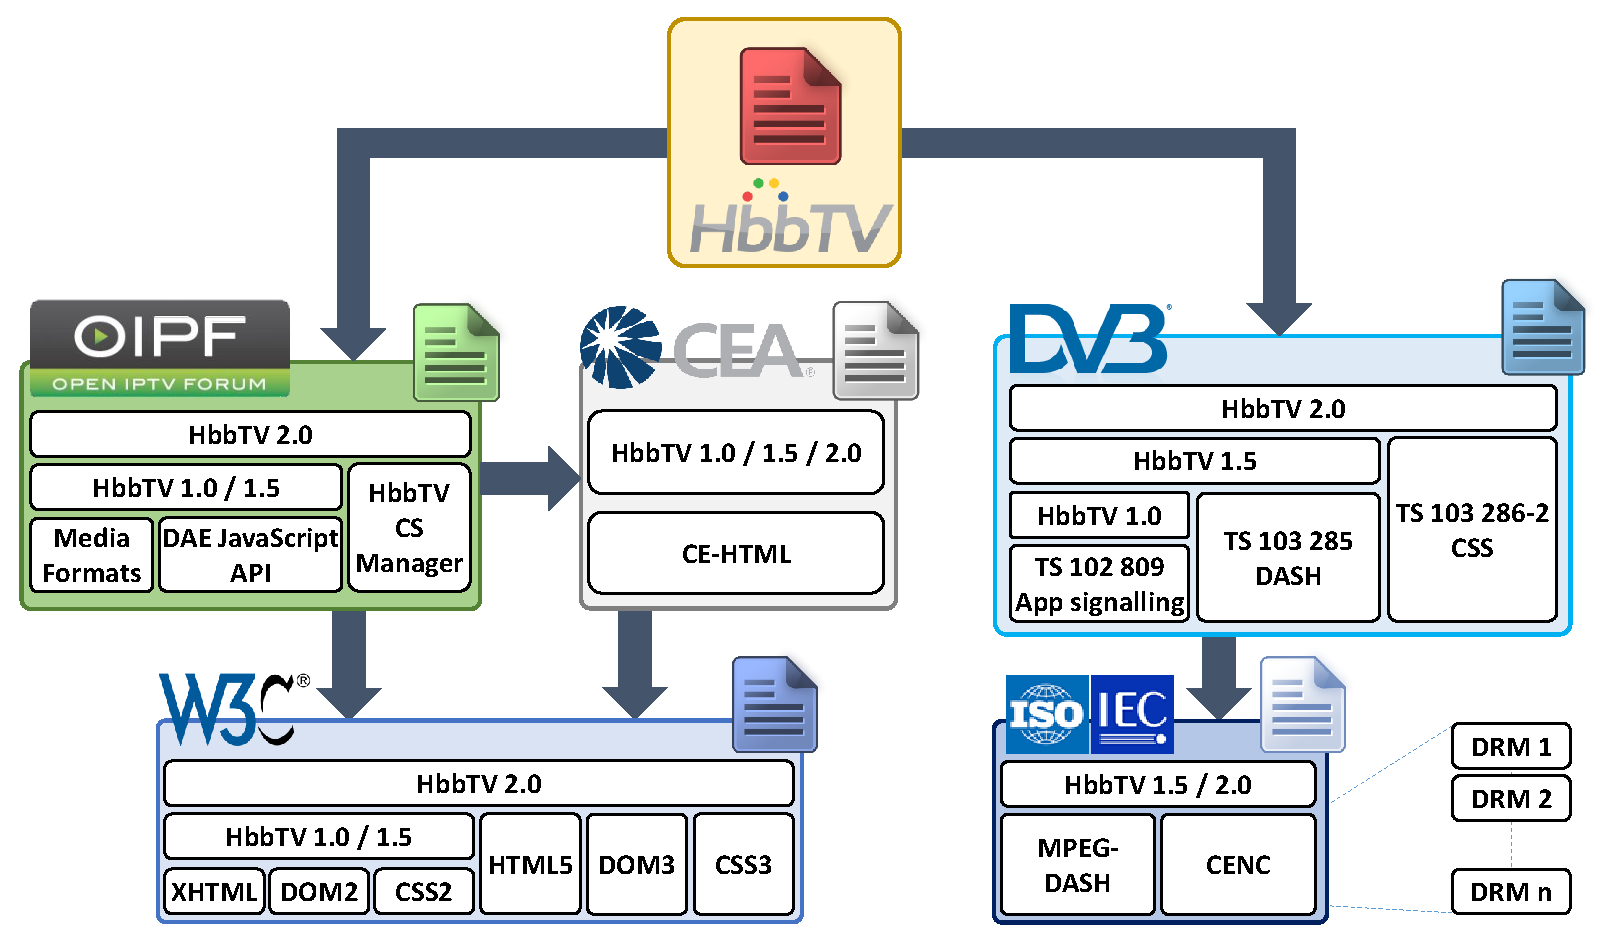
\includegraphics[width=1\textwidth]{hbbtvoverview_cropped}
	\caption{HbbTV overview focused on multi-device services}
	\label{fig:hbbtvoverview}
\end{figure}

Figure \ref{fig:hbbtvoverview} shows the relevant aspects within each block of HbbTV specifications 1.0, 1.5 and 2.0 for the development of HbbTV multi-device services. The Figure extends the HbbTV overview in \cite{hbbtvWeb}, focusing on the multi-screen aspects of the specification and detailing the different features introduced on each one of the HbbTV versions. The Open IPTV Forum (OIPF) \cite{oipf} provides the JavaScript API for TV environments through the Declarative Application Environment (DAE) \cite{DAE}, basing its development on World Wide Web Consortium (W3C) \cite{w3c} specifications, as well as also defining the media formats. Furthermore, latest HbbTV 2.0 specification includes Companion Screen features to discover, launch and communicate second screen devices with the TV in local home networks. More specifically, HbbTVCSManager embedded object is the responsible for discovering the Companion Screens with a running Launcher and sending application launch/install information to them. In the same way, it responds to discovery requests from Companion Screens and launches HbbTV applications in the hybrid terminals. Additionally,  HbbTVCSManager is responsible for providing service endpoints for application to application communication feature. The Consumer Electronics Association (CEA) \cite{cea} defines the application languages (HTML \cite{html}, CSS \cite{css} and JavaScript \cite{js} including AJAX \cite{ajax}) established by W3C as well as the DOM \cite{dom} event handling. A significant change is appreciated in W3C's block from HbbTV 1.5 to HbbTV 2.0, where supported features evolve from XHTML, DOM2 and CSS2 to DOM3, CSS3 and HTML5. These features are supposed to be an enormous benefit for HbbTV multi-device services but commercial devices with full HbbTV 2.0 implementations are not available yet. DVB \cite{DVBstandards} is the one that allows application signalling and its transport via broadcast or HTTP. Moreover, the latest HbbTV 2.0 specification enables the identification and synchronisation of timed content and event triggering between hybrid terminals and personal devices through Companion Screens and Streams (CSS) interface. Finally, the International Organisation for Standardisation (ISO)/International Electrotechnical Commission (IEC) \cite{iso} \cite{iec} provides compatibility with leading Digital Rights Management (DRM) and support for the MPEG-DASH \cite{dash} adaptive streaming.

Furthermore, Operator Applications (OpApps) \cite{opapp} specification is an extension to the core HbbTV specification to support operator application. It describes how the HbbTV browser can run both HbbTV broadcaster applications and operator applications at the same time.
 
Finally, Advanced Television Systems Committee (ATSC) \cite{ATSCWeb} is the group in charge of the development of the Digital TV in USA, Canada, South Korea and Mexico \cite{Chernock2016}. ATSC has launched its 3.0 version \cite{ATSC3} which has been designed to offer support for newer technologies, including HEVC for video channels of up to 2160p 4K resolution at 120 frames per second, wide color gamut, high dynamic range, Dolby AC-4 and MPEG-H 3D Audio, datacasting capabilities, and more robust mobile television support. The new standard is built to have interaction with second devices, providing opportunity to broadcasters to engage on consumers’ devices as well as the TV. The first major deployments of ATSC 3.0 occurred in South Korea, with the country's major television networks launching terrestrial ATSC 3.0 services in May 2017 in preparation for the 2018 Winter Olympics.

These broadcast-related standards, even though they allow mechanisms to launch applications on a companion screen or provide cooperative multi-device application, they do not avoid specific developments for each compatible TV. Moreover, developers have to define the behaviour of the application on each device at the development stage, specifying how to visualise the application on the TV and on the second screen. Developers typically need also to handle the communication between the devices, usually limited to a local network communication, for the contextual synchronisation of the experience.

\section{Technologies for interoperable multi-device services} \label{mdTech}
This subsection presents the available technologies to create interoperable multi-device services. The development of this kind of services is directly related with three main challenges as stated in \cite{thesisMikel}.

\begin{itemize}
	\item Multi-connection: The application itself has to discover the services and other available devices, associating multiple devices to a single user and multiple users to a shared experience, as well as providing mechanisms for a cross platform authentication.
	\item Cross device synchronisation: All the content has to be perfectly synchronised across different devices, taking into account all the media sources, as well as the associated data.
	\item Multi-device adaptation: The application itself has to be adapted to the end-user's dynamic multi-device context, providing a single experience through multiple devices at the same time.
\end{itemize}

If these three challenges are overcome, a versatile and interoperable solution is obtained, independent from the specific target device or platform. The following subsections present the technologies available to face each of the previous challenges.

\subsection{Discovery and association}
When connectivity has to be provided between different devices in an entertainment environment, it is essential to avoid the human intervention as much as possible and make easier the discovery of new services and the association of devices. Nowadays, these are the existing technologies for discovery and association of devices.

\begin{itemize}
	\item Bluetooth: a wireless technology for data exchange in short distances. Bluetooth protocols simplify the discovery and configuration of the services between devices. Bloetooth devices can announce all the services they offer with a high level of security.
	\item NFC: a set of standards for smart phones and similar devices to establish radio communications in a proximity context. Typical applications include wireless transactions, data exchange and simplified configuration of more complex communications such as WiFi.
	\item QR code: Quick Response (QR) is the registered brand of a barcode type designed to store data such as an URL in an efficient way. Its success is due to the easiness to read it and a higher storage than the traditional barcodes. It is commonly used in second screen applications.
	\item Acoustic patterns: acoustic patterns can be emitted by a device to be captured by the surrounding devices. An URL could be mapped to different inaudible frequencies, creating an acoustic code in order to associate two devices. 
	\item Named Web Sockets: Named WebSockets \cite{nws} is an especification that defines the mechanisms to discover and connect pairs of WebSockets that share the same name of service in a local network. The evolution of Named WebSockets is known as Network Web Sockets \cite{netWS}.
	
\end{itemize}

\subsection{Synchronisation}


Media synchronisation has been a key research area since the early development of distributed multimedia systems. A study carried out in \cite{ziegler2017time} shows that users do not notice delays of up to 1000 ms, but they feel significantly more distracted by the second screen content for increasingly higher delays, making the experience less attractive. In this context, \cite{boronat2017hybrid} emphasises the importance of including a combination of media synchronization solutions to guarantee a satisfactory level of Quality of Experience (QoE).

Given the commercial interest in media synchronization and the disadvantages of proprietary technologies, consumer-equipment manufacturers, broadcasters, and telecom and cable operators have started developing a new wave of international standards for media synchronization \cite{van2016standards}. \cite{montagud2018mediasync} provides an approachable overview of media synchronisation from different perspectives, gathering contributions from the most representative and influential experts. 

Concerning the hybrid ecosystem, \cite{boronat2017hbbtv} presents an end-to-end platform for the preparation, delivery and synchronized consumption of related hybrid (broadcast/broadband) media contents on a single device and/or on multiple close-by devices (i.e., a multi-device scenario). It is compatible with the latest version of the Hybrid Broadcast Broadband TV (HbbTV) standard (version 2.0.1).

Regarding Web platform, in order to achieve the synchronisation among devices, W3C through the \textit{Multi-device Timing Community group} \cite{timingComGr} proposes the standardisation of temporal objects called \textit{Timing Object}, to build a model that allows an accurate synchronisation and time controlling in Web-based multi-device applications. It consists on instantiating a timing object in each device that is connected to a online shared temporal source. In order to obtain a perfect synchronisation, the Timing Object supports any velocity and acceleration and any jump in the timeline.

Built on top of the previous work, \textit{timingsrc} \cite{tsrc} can be found which is a programming model based on Timing Objects in order to achieve an accurate synchronisation in multi-device Web applications. Within this model three different services can be found:
\begin{itemize}
	\item MediaSync \cite{mediasync}: it allows the synchronisation of HTML5 videos through a JavaScript library and it is based on a study of the behaviour of media elements in different browsers.
	\item Sequencer \cite{sequencer}: a generic tool to process temporal data. It provides entry and exit events for data used with Timing Objects. 
	\item Shared Motion \cite{shmotion}: it provides an online service to distribute the time to different Web agents. 
\end{itemize}




\subsection{Adaptation}


There are available solutions and in-progress language recommendations in the field of adaptive interface of Web applications and its responsive design addressing the adaptation for a single device. However, these approaches do not face the adaptation of an application in the multi-device domain.

Responsive Web design is a key factor in Web development, targeting devices with different features such as connected TVs, laptops, tablets and mobiles. Their heterogeneous displays and characteristics requires the responsive Web design to provide an adequate viewing experience automatically adapted for each device.

HTML features a number of fall-back mechanisms to adjust the content to the device capabilities. Two different approaches to design responsive Web applications can be deployed. On the one hand, a server-side detection based upon information embedded in HTTP requests. The result can be used to return a suitable media content, e.g. a video, where the server selects an optimal bitrate and resolution mode for the requested content based on the device in question.

The second approach for responsive Web applications, covered by the HTML mechanisms, is based on client-side detection and adaptation, enabling a wider set of possibilities. HTML5 includes attributes (\textit{srcset}) that allow application developers to provide multiple resources in varying resolutions for a single image \cite{W3C2014HTML}. Audio and video tags (\textit{<audio>}, \textit{<video>}) permit the definition of different source types and let the browser choose which format to use on the current device (audio/ogg, audio/mp3, etc.). Another powerful client-side mechanism is based on \textit{media queries (@media)} \cite{W3C2012MQ}. These simple filters can be applied to CSS styles in order to change the properties based on characteristics of the end-device. Even for showing suitable media content at the client, the trend with streaming protocols like MPEG-DASH moves the adaptation from the server to the client.

Nevertheless, the most widespread way to achieve adaptive interfaces lays on designing the CSS style sheets to be applied to different displays. Therefore, the alternatives often match the application design with the device context, adapting the layout and the user interface. W3C proposes some basic recommendations \cite{W3C2010WA} to improve the user experience of the Web when accessed from mobile devices.

There are several frameworks that support the development of responsive applications. Gridster.js \cite{gridster}  boosts the dynamic grid layouts for drag-and-drop actions based on jQuery. CSS3 Flexbox \cite{W3C2014FB} empowers the layout definition in the CSS by describing a box model optimised for the user interface design, where the children of a flex container can be laid out in any direction –both horizontal and vertical – in a flexible way. CSS3 Regions \cite{W3C2014Reg} allows elements moving through different regions where CSS Regions library \cite{cssreg} expands the browser support with broader feature coverage. Grid-layout \cite{W3C2014GL} defines a two-dimensional grid-based layout system, optimised for user interface design. The XML XUL\cite{mozxul} language has been created by Mozilla to design user interfaces. Kontx \cite{kontx} is the proposal of Yahoo to develop TV apps. EnyoJS \cite{enyo} is a framework to develop HTML5 apps focused on layouts and panels design. Bootstrap \cite{bootstrap} is a framework for developing responsive mobile-first projects on the Web that includes a grid system to scale the layout as the device or viewport size changes.

Web Components \cite{webcomps} is the umbrella term for a set of new W3C specifications that give developers the primitives needed to build reusable and interoperable elements. The individual specifications that make up Web Components map almost directly to the specific features needed to create a truly interoperable element.
\begin{itemize}
	\item The Custom Elements specification \cite{customelements} describes how an element might be given a name, define an API surface area, and respond to different events in its lifecycle. That way, personalised elements can be easily reused in different web applications.
	\item The HTML5 <template> element \cite{htmltemplate} provides the set of features needed to declare inert DOM subtrees ready to be instantiated in the final DOM.
	\item The Shadow DOM spec \cite{shadowdom} provides the mechanism for encapsulation. It introduces the notion of a "Shadow Root" which is a separate, scoped tree that mantains functional boundaries between DOM trees and avoiding, for instance, accidental interference by CSS selectors or DOM manipulation methods.
	\item The HTML Imports specification \cite{htmlimports} provides this mechanism to load HTML-based dependencies in HTML.
	
\end{itemize}

With these four crucial new features Web developers are provided with the platform-level primitives needed to create truly reusable custom elements, with all the power of native HTML elements.

The JavaScript implementations of the previous specifications support Custom Elements, HTML Imports, and Shadow DOM across the last two versions of major browsers starting with IE10, Safari 7, and the evergreen browsers Chrome and Firefox. Moreover, Web Components-based libraries such as X-Tag \cite{xtag}, Polymer \cite{polymer}, and Bosonic \cite{bosonic} rely on some of the polyfills\footnote{A polyfill is a downloadable code which provides facilities that are not built natively in a Web browser} for broad browser support, and include optimisations around the heavier parts of the polyfills to achieve production-ready performance.

Apart from Web Components, other frameworks such as Angular or React also allow component-based Web development. These frameworks are not based on any standard and therefore, they present less dependencies. 

The combination of components and \textit{media queries} boost the development of responsive multi-device Web applications and they are core technologies, among others, of the next generation of Google apps \cite{T2013G}.

All these languages, recommendations and frameworks for adaptive interfaces and responsive design are very useful for smooth local adaptation but need to be extended towards the multi-device dimension. They are all designed to adapt an application to a device aiming the adaptation depending on the device features. However, they do not consider that an application can be running in one or more devices simultaneously, including only part of the application.

\section{Optimisation of user interface of multi-device media services} \label{UIOpt}
This subsection describes the attempts to optimise the user interface of multi-device media services found in the literature. Optimisation methods have been a long-standing topic in HCI research for user interface (UI) design. Nevertheless, these optimisation methods have been explored as supplemental ways to help speed up the design cycle and improve the design quality. Theoretically, model-based UI optimisation refers to the use of combinatorial methods to solve a UI design problem formulated as a search problem by using predictive models of human behaviour and experience \cite{oulasvirta2017user}. However, to the best of our knowledge, no existing adaptation models are available to dynamically and seamlessly adapt such a multitude of content to multi-device and multi-user contexts, where a user or a group of users consumes content from a set of devices at the same time.

With the advent of the aforementioned new and interactive media experiences, Layout Appropriateness (LA) \cite{sears1993layout} has become a key term for the evaluation of user interfaces. The LA concept assigns a cost to every layout according to specific metrics such as the time required to accomplish a task or the users' preferences. Therefore, the appropriateness of a given layout is computed by weighting the cost of each sequence of actions and seeing how frequently the sequence is performed. In this context, Sketchplore \cite{todi2016sketchplore} is defined as the first user interface optimiser that uses different metrics to optimise the spatial and colour aspects of interactive layouts. 

%However, due to the great dynamism of a multi-device system where a single user can be consuming content from multiple screens at the same time, the typical template-based approach is not valid in order to arrange the set of elements to be shown in each device and to decide how to show them.
However, in a multi-device system where a user can be consuming content from multiple screens at the same time, the typical template-based approach cannot work, as the set of elements to be shown on each device can change over time, depending on the number of components to visualise and the number of devices connected to the system.
In a multi-screen environment, such as that addressed in \cite{Zorrilla2015}, the content is divided into logic elements with the Web components specification \cite{webcomps} following an object-based broadcasting approach \cite{armstrong2014object}. In this context, the system will dynamically decide which elements of the application will be shown on each device, simultaneously splitting the application through different devices, to provide a consistent and coherent view to the user, which means that the list of elements available on each device will depend on the changeable context of the users and will dynamically update when a new device is added or removed. In this scenario, it is tedious, very expensive and unaffordable for developers to provide an explicit template to organise the elements on the user interface of each target device, considering all the possible combinations. Thus, the solution described in \cite{Zorrilla2015} provides generic and arbitrary divisions to arrange the elements in a responsive user interface following some hints given in the application code and creates a specific layout template depending on the context of the user.

Regarding cross-device adaptation, \cite{brudy2019cross} aimed to create a unified terminology to facilitate cross-device research; \cite{dong2016understanding} identified technological and business factors that represent a barrier to create useful, usable and delightful multi-device experiences; \cite{grubert2016challenges} presented the relevant challenges for the design, development and use of mobile multi-device environments; \cite{santosa2013field} provided a field study of multi-device workflows in distributed workspaces; \cite{waljas2010cross} revealed the key elements of the user experience associated with cross-platform interactions and proposes an initial conceptual framework that can be used to guide the design of cross-platform web-services; \cite{bbcExp} explored how second screens might enhance live TV shows with additional web content and external links; and \cite{jokela2015diary} provided a user study on people's current practices in combining multiple devices in their everyday lives. 

Apart from the previous studies and the identification of challenges, the XDBrowser \cite{nebeling2017xdbrowser} \cite{nebeling2016xdbrowser} project investigates how web browsers can be improved to better support parallel multi-device usage and provides a proof-of-concept implementation that segments web pages and distributes the parts across devices. Webstrates \cite{klokmose2015webstrates} synchronises elements across devices operating on the level of the Document Object Model (DOM) while maintaining exact copies on different devices. \cite{sarkis2018multi} allowed for the re-use of existing single-screen applications to automatically create synchronous multi-screen applications that analyse the code of the application and classifies different elements, such as HTML tags or event listeners. Other frameworks work with graphical aspects of user interfaces, for instance, when spanning one image across multiple screens \cite{radle2014huddlelamp} \cite{schreiner2015connichiwa}. Other prior works on cross-device interfaces, such as \cite{frosini2014user} or \cite{yang2014panelrama}, have proposed methods for synchronising elements across devices. All of these frameworks allow for the development of new multi-screen applications but they all require developers in the development stage to explicitly define how to distribute interface components across displays.

There are also rule-based approaches, such as \cite{husmann2017orchestrating} or \cite{nebeling2017xdbrowser}, which provide insights into cross-device interaction patterns. However, they are focused on very specific functionalities and do not scale to many devices or multi-user scenarios. Vistribute \cite{horak2019vistribute} proposes a framework that identifies important properties and relations for distributed visualisation interfaces. Vistribute also provides six heuristics that can guide in the automatic distribution of visualisations in changing device setups together with their web-based implementation. However, those heuristics are focused on data analysis visualisations and therefore they are again not general enough to extend them for the adaptation of other contents in different fields.

AdaM \cite{park2018adam} proposed an optimisation-based approach that automatically distributes elements to available devices by solving the many-to-many assignment problem. AdaM distributes the UI elements based on an objective that maximises the usefulness of an element on a device while simultaneously maximising the completeness of the UI form from the user's perspective. However, the problem of a layout of elements on a device is not addressed in this work, as it is assumed to be performed via responsive design practices common in web design.

In the mentioned literature there is a lack of an adaptation model that takes into account the following aspects:
\begin{itemize}
	\item Ability to distribute and adapt such a dynamic amount of content to any device.
	\item Good performance at run-time and in real-time without having a negative effect in the user experience.
	\item Usefulness for any multi-device and multi-user context.
	\item Provision of a systematic basis for the adaptation that frees the developer from the duty of defining a wide range of explicit rules. 
\end{itemize}

However, the definition of the model itself is not straightforward, which is why this work proposes a methodology to adapt the user interface of multi-device media services. 








